\section{Problema II: Problemas en el camino}

\subsection{Introducción}

%Explicación informal
En este ejercicio, el grupo de arqueólogos necesita abrir una puerta cerrada con llave. En la misma habitación hay una balanza con dos platillos, y sobre uno de los platillos se encuentra la llave de la puerta. Al sacar la llave de la balanza, ésta cambia su equilibrio, la puerta se cierra y las paredes comienzan a moverse hacia ellos con el fin de aplastarlos. Para frenar las paredes y poder usar la llave, los arqueólogos tienen que volver la balanza a su equilibrio inicial utilizando un conjunto de pesas (ya que necesitan la llave como para volverla a colocar en la balanza), que tienen como peso una potencia de tres (no hay pesas del mismo peso). Para la suerte de los arqueólogos, uno de ellos tiene una balanza digital que les indica el peso de la llave que deben restablecer.

%Conectar la explicación informal con la formal
Dicho de forma más formal, dado el peso de la llave, se debe restablecer la balanza, de forma tal que la sumatoria de los pesos que se coloquen en el platillo donde estaba la llave, restada a la sumatoria de los pesos que se coloquen en el otro platillo, sea equivalente al peso de la llave.



\subsection{Resolución del problema}

Como los pesos en ambos platillos son sumatorias de potencias de 3, decidimos representar el peso de la llave como un número escrito en base 3. Este número nos dice que el valor $a_i$ del número, siendo $i$ la posición del valor comenzando a contar desde el valor menos significativo, es la constante que multiplica a la potencia $3^i$, el cual puede ser $0,\ 1\ o\ 2$. Estas constantes nos van a servir para saber qué pesas tenemos que utilizar en qué balanza. Por cada dígito de la representación del peso de la llave en base 3 tenemos que tomar una decisión según su valor. Entonces tenemos 3 casos distintos:

\begin{itemize}
    \item \textbf{$a_i = 0$: } 
        Este caso indica que no tenemos que poner ninguna pesa en ningún platillo. Como esta potencia de 3 no esta incluida en la sumatoria de potencias de 3 que representa al peso de la llave, no tenemos que agregarla a la balanza.
        
    \item \textbf{$a_i = 1$: } 
        Este caso indica que tenemos que poner la pesa de peso $3^i$ en el platillo donde se encontraba la llave. Esto se debe a que la potencia $3^i$ se encuentra en la sumatoria de potencias de 3 que representa al peso de la llave. 
    
    \item \textbf{$a_i = 2$: } 
        Este caso indica que deberíamos agregar peso para tratar de compensar la sumatoria, pero como solo tenemos un peso de cada potencia de 3, no podemos agregar 2 pesos en el platillo en que estaba la llave. Por eso es que agregamos el peso $3^i$ en el otro platillo y sumamos el valor $3^i$ representado en base 3, al peso de la llave representado también en base 3. Esto equivale a sumarle 1 a $a_i$, que quedaría en 0 y se le suma 1 al valor $a_{i+1}$ (incluyendo también que todos los valores siguientes de la representación sean menores a 3).
        
        Sabemos que esto funciona por la siguiente igualdad:
        $3^{i+1} = 3*3^i = 2*3^i + 3^i$.
        En términos de nuestro problema, $2*3^i$ es el valor que nosotros tenemos y no podemos poner el el platillo de la llave. Entonces si le sumamos el término $3^i$ (es decir, ponemos el peso $3^i$ en el otro platillo para aumentar el peso que tenemos que poner en el platillo de la llave), necesitaríamos agregar el peso $3^{i+1}$ al platillo de la llave. 
        
\end{itemize}

Como se puede observar en el último de nuestros casos, para evitar problemas por sumarle 1 al valor $a_{i+1}$, tenemos que analizar este valor luego de analizar todos los valores menos significativos antes para tener los valores posteriores que serán usados efectivamente.

Sabiendo como operar con cada dígito de la representación en base 3 del peso de la llave, procedemos a armar nuestro algoritmo. Éste consiste en iterar sobre cada dígito de la representación, del valor menos significativo hasta el más significativo, y para cada dígito realizar alguno de los 3 casos descriptos previamente. 

Para facilitar los cálculos, cuando ``nos llevamos una'', establecemos una variable booleana como verdadera para indicarnos que en la siguiente iteración tenemos que sumarle 1 al valor.

A continuación incluimos el pseudocódigo del algoritmo:


\subsection{Pseudocódigo}

\begin{algorithm}[h]
\caption{resolver}
\begin{algorithmic}[1]
  \Procedure{resolver}{int peso\_llave} $\to $ \texttt{List<int> platillo\_llave, List<int> platillo\_otro}
  
  
    \State \textbf{//Obtengo la representación en base 3. De valores menos significativos a más significativos.}
	\State \texttt{List<Integer>} key\_weight\_base\_3 $\gets$ toBase3(peso\_llave);	
	
	\State
    \State \textbf{//Booleano para saber si me lleve una o no.}
	\State boolean iTookOne = false;					
	
    \State 
    \For{(int i = 0; i $<$ key\_weight\_base\_3.length; i++)}

		\State \textbf{//Obtengo el valor i de la representación de la base.}
		\State int value = key\_weight\_base\_3.get(i);		
		
		\State 
		\State \textbf{//Si me lleve una antes incremento el valor.}
		\If{(iTookOne)}
		
			\State value++;				
			\State iTookOne = false;
			
		\EndIf
		
		\State 
		\State \textbf{//Agrego las pesas en los platillos correspondientes.}
		\If{(value == 0)}
		
			%\State 
			\State \textbf{//No tengo que poner ninguna pesa.}
			\State 
			
		\ElsIf{(value == 1)}
	
		    %\State 
			\State \textbf{//Tengo que poner la pesa $3^i$ en el lado de la llave.}
			
		    \State platillo\_llave.add($3^i$);
		    \State 
		\ElsIf{(value == 2)}
			
			%\State 
			\State \textbf{//Tengo que poner la pesa $3^i$ en el otro lado y me llevo una para compensar los pesos.}
				
			\State platillo\_otro.add($3^i$);
			\State iTookOne = true;	
			\State 
			
		\Else
			%\State 
			\State \textbf{//No tengo que poner ninguna pesa. Me llevo una para compensar.}
			\State \textbf{//(valor == 3, entonces la consideramos como 0 y me llevo una).}
			
			\State iTookOne = true;
			
		\EndIf	
	
	\EndFor
	
 \EndProcedure
 
\end{algorithmic}
\end{algorithm}



\newpage

\begin{algorithm}
\caption{toBase3}
\begin{algorithmic}[1]
  \Procedure{toBase3}{int peso\_llave} $\to $ \texttt{List<int> base3}
 
		\While{ (peso\_llave $>$ 0) }   		
		
		    \State \textbf{//Obtengo cociente y resto.}
			\State int quotient  = peso\_llave / 3;
			\State int remainder = peso\_llave \% 3;
			
			\State
			\State \textbf{//Actualizo el peso de la llave.}
			\State peso\_llave = quotient;				
			\State
			\State \textbf{//Agrego el valor a la lista resultado.}
			\State base3.add( remainder );		
		
		\EndWhile
		
		\State
		\State return base3;
	
		
		\EndProcedure
 
\end{algorithmic}
 
\end{algorithm}


\subsection{Correctitud}

En esta sección explicaremos por qué el algoritmo funciona. Sabemos que todo número puede representarse como una sumatoria de potencias de una misma base $b$, donde cada potencia puede ser multiplicada por un número menor a $b$. Es decir, para nuestro caso podemos expresar el número $X$ como una sumatoria de potencias de $3$ multiplicadas por un valor  $ 0 \leq a_i \leq 2$: 
\[
\sum_{0}^{\infty}a_i*3^i = X
\]

Si consideramos al término izquierdo de la igualdad como el platillo de la balanza donde se encontraba la llave, y al término derecho de la igualdad como el otro platillo de la balanza, nuestro algoritmo lo que hace es transformar la sumatoria en otra sumatoria de potencias de $3$ pero el valor que multiplica a cada potencia va a ser solamente el valor $0$ o $1$. El valor $X$ de este lado se utiliza simplemente para representar el equilibrio inicial en la balanza y simplificar las cuentas y explicaciones.

Esto lo logramos transformando a las potencias $3^i$ multiplicadas por el valor $2$, en potencias $3^{i+1}$. La transformación se basa en la igualdad $3^{i+1} = 3*3^i = 2*3^i + 3^i$. Usando esta igualdad podemos, escribir al término $2*3^i$ como $3^{i+1}$, siempre y cuando compensemos el término $3^i$ en el otro lado de la igualdad.

Obtenido el término $3^{i+1}$, tenemos 3 casos que analizar: 

\begin{itemize}
    \item \underline{ \textbf{En la sumatoria original, $a_{i+1} = 0$ o $a_{i+1} = 1$: } } En estos casos sumamos el término obtenido en la transformación, y obtenemos que el valor que multiplica a la potencia $3^{i+1}$ ahora es $1$ o $2$. Siendo estos dos los valores que quedan multiplicando a la potencia, podemos proceder a continuar con el algoritmo, el cual manejara a estos valores cuando le toque analizarlos.
    
    \item \underline{ \textbf{En la sumatoria original, $a_{i+1} = 2$: }} En este caso, al sumarle la potencia $3^{i+1}$ obtenida en la transformación, se obtiene el término $3*3^{i+1}$, que es equivalente a $3^{i+2}$. A este nuevo valor lo podemos sumar al término $i+2$ de la sumatoria, teniendo que analizar nuevamente estos 3 casos para ese término.
   
\end{itemize}

Estas últimas operaciones terminan en algún momento, dado que no hay términos infinitos de la sumatoria que tengan $a_{k} = 2$ como valor que multiplica a la potencia $3^k$.

Explicada la razón de porque transformar la sumatoria de la igualdad, nos falta justificar que al terminar de iterar los términos de la sumatoria desde el más chico hasta el más grande, no nos quedan potencias de $3$ con el mismo exponente en ambos lados de la igualdad.

Esto se ve fácilmente de la siguiente forma: cuando estamos iterando el término $i$ de la sumatoria, todos los términos anteriores (que van a ser potencias más chicas que la actual), ya fueron analizadas, y los resultados de estas implicaron que no haya término $3^j$ ($j<i$) en ningún lado de la igualdad, que el término $3^j$ esté del lado izquierdo de la igualdad con $a_j = 1$, o que $3^j$ esté del lado derecho de la igualdad también con $a_j = 1$. Esto nos asegura que al menos hasta la iteración $i$, tenemos a lo sumo solo una potencia $3^i$ entre ambos lados de la igualdad.

Con respecto a los término siguientes a $i$, como mantenemos los valores $a_l$ ($l>i$) iguales a $0,~1~ o~ 2$, siempre van a estar en condiciones de ser resueltos correctamente por iteraciones siguientes del algoritmo.

Una vez que el algoritmo termina, lo que obtenemos es una igualdad de la forma:
\[
\sum_{0}^{\infty}a_i*3^i = X + \sum_{0}^{\infty}b_i*3^i
\]

para las cuales $0 \leq a_i \leq 1$, $0 \leq b_i \leq 1$ y $a_i + b_i \leq 1 $ (es decir que sólo esta la potencia $1*3^i$ en a lo sumo uno de los lados de la igualdad).

Como dijimos al comienzo, el lado izquierdo se corresponde con el platillo donde se encontraba la llave, y el lado derecho de la igualdad se corresponde con el otro platillo. Entonces, por cada término $1*3^i$ del lado izquierdo de la igualdad, tenemos que poner la pesa del mismo valor en el platillo. De forma análoga para el lado derecho, agregamos los valores $1*3^i$ de la sumatoria como pesas del mismo valor en el platillo.

\subsection{Complejidad del algoritmo}

Comenzaremos por la complejidad de la función toBase3(peso). Esta función devuelve la representación en base 3 del número pasado como parámetro y consiste en un ciclo donde las operaciones que se hacen tienen tiempo constante. Estas operaciones son de dividir el número por 3 hasta que el resultado sea 0 y obtener el resto, valor que será un elemento de la representación en base 3 del número. Entonces la complejidad de la función será la cantidad de veces que itere el ciclo. La cantidad de iteraciones que realiza será luego la parte entera superior del logaritmo en base 3 del peso. En la siguiente ecuación buscamos la cantidad de veces que debe iterarse la división para que peso sea menor a 1 (es decir, sea 0):
\[ 
peso/(3^x) < 1 
\] \[
peso < 3^x
\] \[
log_3(peso) < log_3(3^x)
\] \[
log_3(peso) < x
\]

Siendo X la cantidad de veces que dividimos el peso por 3, se ve que X tiene que ser mayor al $log_3$ del peso. Como X es un valor entero, nuestro X será el valor entero superior de $log_3(peso)$.

Como la cantidad de elementos de la lista retornada es uno por cada iteración, la cantidad va a ser también el valor entero superior inmediato a $log_3(peso)$.


Sabiendo esta complejidad, podemos explicar la complejidad de la función resolver(peso). Como se puede observar en el pseudocódigo, todas las operaciones que se realizan son operaciones de tiempo constante. Entonces lo que va a determinar la complejidad del algoritmo es la complejidad de la llamada a la función toBase3(peso) y la cantidad de iteraciones que realiza el ciclo. Este ciclo itera sobre cada uno de los elementos de la representación del número devuelta por la función toBase3(peso). Es decir que va a iterar $log_3(peso) +1$ veces, una por cada dígito de la representación en base 3 de nuestro número, con todas operaciones constantes en cada iteración. 

Sumando las complejidades importantes, tenemos por la llamada a toBase3 la complejidad $log_3(peso)$, y por el ciclo tenemos la misma complejidad.

Luego, la complejidad del algoritmo va a ser $O(log_3(peso))$. Como esta complejidad es menor a $\sqrt{peso}$, cumple con la condición pedida de que la complejidad debe ser menor a $O(\sqrt{peso})$.

\newpage
Mostremos ahora que $O(log_3(x))$ es menor a $O(\sqrt{x})$.

\[
log_3(x) < \sqrt{x}
\] \[
0 < \sqrt{x} - log_3(x)
\]
Derivando $f(x) = \sqrt{x} - log_3(x)$ obtengo :
\[
f'(x) = 1/2\sqrt{x} \ - \ 1/x.ln(3)
\] \[
f'(x) = (1 - 2/\sqrt{x}.ln(3)) \ /2\sqrt{x}
\]

Como puede observarse la derivada es positiva cuando $1 - 2/\sqrt{x}.ln(3)$ lo es. Luego:
\[
1 - 2/\sqrt{x}.ln(3) > 0
\] \[
1 > 2/\sqrt{x}.ln(3)
\] \[
\sqrt{x} > 2/ln(3) \approx 1.82
\]

Y esta desigualdad se cumple cuando $4 \leq x$.
 
De esta forma obtenemos que $f(x) = \sqrt{x} - log_3(x)$ es creciente $\forall x \geq 4$. Calculando $f(4)$:
\[
f(4) = \sqrt{4} - log_3(4) \approx 2 - 1.26185950714291 > 0 \ \forall \ x \geq 4
\]
y como $f(x)$ es creciente, tenemos que 
\[
f(x) > 0 \ \forall x \geq 4
\] \[ 
\sqrt{x} - log_3(x) > 0 \ \forall x \geq 4
\] \[
\sqrt{x} > log_3(x)  \ \forall x \geq 4
\]

Analizando los valores $x = 1,2,3$:

\[
\sqrt{1} = 1 > log_3(1) = 0
\] \[
\sqrt{2} > 1.4 > 0.64 > log_3(2)
\] \[
\sqrt{3} > 1.7 > log_3(3) = 1
\] 

Luego obtuvimos:
\[
\sqrt{x} > log_3(x)  \ \forall x > 0
\]
Y por ende:
\[ 
O(log_3(x)) es menor que O(\sqrt{x})
\]


 

\newpage
\subsection{Experimentación}

Como el único parámetro de entrada del algoritmo es P, como experimentación correremos el programa variando el P en instancias pequeñas e instancias grandes, dado que P puede tomar valores de hasta $10^{15}$.

\begin{figure}[H]
    \centering
    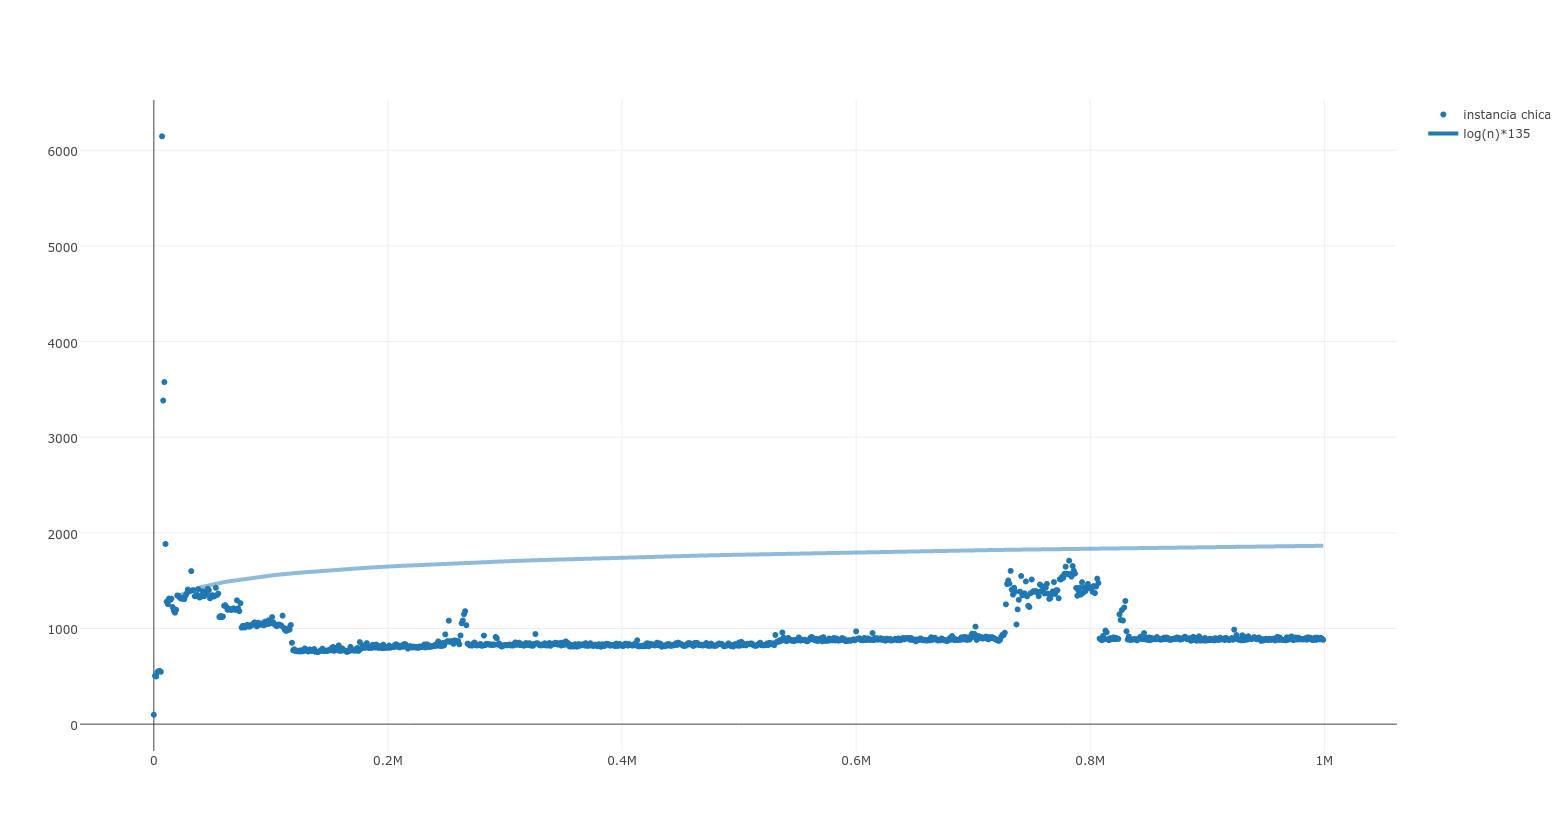
\includegraphics[width=\textwidth]{./imagenes/ej2chico.png}
    %\caption{FCFS con 2 núcleos}
    %\label{fig:my_label}
\end{figure}

Si bien en el gráfico los resultados estan por debado de la función log(P).350, se puede observar que el crecimiento del tiempo de la ejecución de las instancias es muy leve. Esto se debe a que en realidad el algoritmo tiene como complejidad al entero superior próximo de $log_3(x)$. Además, al ser un logaritmo, la instancia más grande da que $log_3(1.000.000)$ $\approx$ 12.6, y para una instancia no tan chica, digamos 100.000, tenemos que $log_3(100.000) \approx 10.5$. Por lo que al ser tan pequeña esta diferencia, ya que los valores enteros de los logaritmos varían entre 11 y 13 (por ser el entero superior mas próximo), la complejidad empírica obtenida pareciera tener un comportamiento constante.
%Para las instancias más chicas se obtuvieron valores anómalos. Estos valores se generaron por operaciones que realiza la JVM de las cuales no tenemos control para evitarlos.
%En el gráfico se puede ver que los tiempos obtenidos se encuentran por debajo de la función $log(P)$. Utilizamos la constante 350 para generar un gráfico en el que se pueda apreciar que ambas curvas tienen un comportamiento de crecimiento de estilo logarítmico. 
\\
Las instancias van de 0 a 1 millón.


\begin{figure}[H]
    \centering
    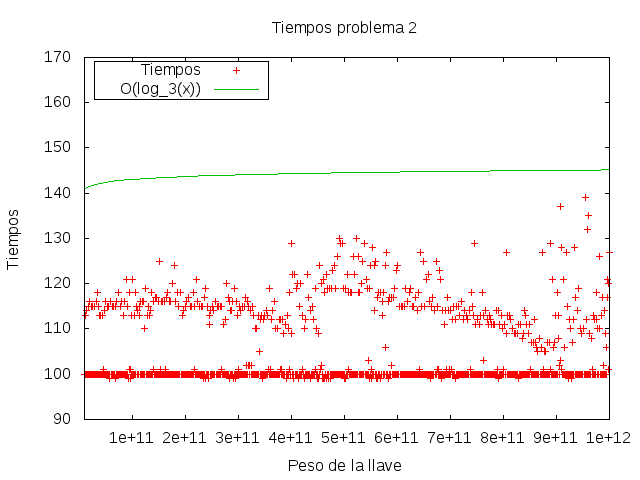
\includegraphics[width=15cm]{./imagenes/tiemposEj2.png}
    %\caption{FCFS con 2 núcleos}
    %\label{fig:my_label}
\end{figure}


En el siguiente gráfico se testearon pesos más grandes desde $10^{10}$ hasta $10^{12}$ y se ve que se cumple con la cota propuesta. Como puede observarse, la mayoría de los tiempos obtenidos en los experimentos tienen un valor similar a la experimentación anterior. Nuevamente esto se debe a que la diferencia entre tiempos al ser una complejidad logarítmica entre distintos tamaños de instancia es muy chica: en estas instancias con valores elevados la curva logarítmica es tan leve que al tomar sus valores enteros superiores se comporta como una recta constante en este rango de instancias.


